\section{Hierarchies of decision making problems}
\only<presentation>{
  \begin{frame}
    \tableofcontents[ 
    currentsection, 
    hideothersubsections, 
    sectionstyle=show/shaded
    ] 
  \end{frame}
}


\only<article>{
  All machine learning problems are essentially decision problems. This essentially means replacing some human decisions with machine decisions. One of the simplest decision problems is classification, where you want an algorithm to decide the correct class of some data, but even within this simple framework there is a multitude of decisions to be made. The first is how to frame the classification problem the first place. The second is how to collect, process and annotate the data. The third is choosing the type of classification model to use. The fourth is how to use the collected data to find an optimal classifier within the selected type. After all this has been done, there is the problem of classifying new data. In this course, we will take a holistic view of the problem, and consider each problem in turn, starting from the lowest level and working our way up.}


\subsection{Simple decision problems}
\begin{frame}
  \frametitle{Preferences}
  \only<article>{The simplest decision problem involves selecting one item from a set of choices, such as in the following examples}  
  \begin{example}
    \begin{block}{Food}
      \begin{itemize}
      \item[A] McDonald's cheeseburger
      \item[B] Surstromming
      \item[C] Oatmeal
      \end{itemize}
    \end{block}
    \begin{block}{Money}
      \begin{itemize}
      \item[A] 10,000,000 SEK
      \item[B] 10,000,000 USD
      \item[C] 10,000,000 BTC
      \end{itemize}
    \end{block}
    \begin{block}{Entertainment}
      \begin{itemize}
      \item[A] Ticket to Liseberg
      \item[B] Ticket to Rebstar
      \item[C] Ticket to Nutcracker
      \end{itemize}
    \end{block}
  \end{example}
\end{frame}

\begin{frame}
  \frametitle{Rewards and utilities}
  \only<article>{In the decision theoretic framework, the things we receive are called rewards, and we assign a utility value to each one of them, showing which one we prefer.}
  \begin{itemize}
  \item Each choice is called a \alert{reward} $r \in \CR$.
  \item There is a \alert{utility function} $U : \CR \to \Reals$, assigning values to reward.
  \item We (weakly) prefer $A$ to $B$ iff $U(A) \geq U(B)$.
  \end{itemize}
  \only<article>{In each case, given $U$ the choice between each reward is trivial. We just select the reward:
    \[
      r^* \in \argmax_r U(r)
    \]
    The main difficult is actually selecting the appropriate utility function. In a behavioural context, we simply assume that humans act with respect to a specific utility function. However, figuring out this function from behavioural data is non trivial. ven when this assumption is correct, individuals do not have a common utility function.
  }
  \begin{exercise}
    From your individual preferences, derive a \alert{common utility function} that reflects everybody's preferences in the class for each of the three examples. Is there a simple algorithm for deciding this? Would you consider the outcome fair?
  \end{exercise}
\end{frame}

\begin{frame}
  \frametitle{Preferences among random outcomes}
  \begin{example}
    Would you rather \ldots
    \begin{itemize}
    \item[A] Have 100 EUR now?
    \item[B] Flip a coin, and get 200 EUR if it comes heads?
    \end{itemize}    
  \end{example}
  \uncover<2->{
    \begin{block}{The expected utility hypothesis}
      Rational decision makers prefer choice $A$ to $B$ if
      \[
        \E(U | A) \geq \E(U | B),
      \]
      where the expected utility is
      \[
        \E(U | A) = \sum_r U(r) \Pr(r | A).
      \]
    \end{block}
    In the above example, $r \in \{0, 100, 200\}$ and $U(r)$ is
    increasing, and the coin is fair.
  }
  \begin{itemize}
  \item<3-> If $U$ is convex, we prefer B.
  \item<4-> If $U$ is concave, we prefer A.
  \item<5-> If $U$ is linear, we don't care.
  \end{itemize}
\end{frame}


\begin{frame}
  \frametitle{Uncertain rewards}
  \only<article>{However, in real life, there are many cases where we can only choose between uncertain outcomes. The simplest example are lottery tickets, where rewards are essentially random. However, in many cases the rewards are not really random, but simply uncertain. In those cases it is useful to represent our uncertainty with probabilities as well, even though there is nothing really random.}
  \begin{itemize}
  \item Decisions $\decision \in \Decision$
  \item Each choice is called a \alert{reward} $r \in \CR$.
  \item There is a \alert{utility function} $U : \CR \to \Reals$, assigning values to reward.
  \item We (weakly) prefer $A$ to $B$ iff $U(A) \geq U(B)$.
  \end{itemize}

  \begin{example}
    \begin{columns}
      \begin{column}{0.5\textwidth}
      You are going to work, and it might rain.  What do you do?
        \begin{itemize}
        \item $\decision_1$: Take the umbrella.
        \item $\decision_2$: Risk it!
        \item $\outcome_1$: rain
        \item $\outcome_2$: dry
        \end{itemize}
      \end{column}
      \begin{column}{0.5\textwidth}
      \begin{table}
          \centering
          \begin{tabular}{c|c|c}
            $\Rew(\outcome,\decision)$ & $\decision_1$ & $\decision_2$ \\ %ro: U has only one argument.
            \hline
            $\outcome_1$ & dry, carrying umbrella & wet\\
            $\outcome_2$ & dry, carrying umbrella & dry\\
            \hline
            \hline
            $U[\Rew(\outcome,\decision)]$ & $\decision_1$ & $\decision_2$ \\
            \hline
            $\outcome_1$ & 0 & -10\\
            $\outcome_2$ & 0 & 1
          \end{tabular}
          \caption{Rewards and utilities.}
          \label{tab:rain-utility-function}
        \end{table}

        \begin{itemize}
        \item<2-> $\max_\decision \min_\outcome U = 0$
        \item<3-> $\min_\outcome \max_\decision U = 0$
        \end{itemize}
      \end{column}

    \end{columns}
  \end{example}
\end{frame}



\begin{frame}
  \frametitle{Expected utility}
  \[
    \E (U \mid a) = \sum_r U[\Rew(\outcome, \decision)] \Pr(\outcome \mid \decision)
  \]
  \begin{example}%ro: rather an exercise?
    You are going to work, and it might rain. The forecast said that
    the probability of rain $(\outcome_1)$ was $20\%$. What do you do?
    \begin{itemize}
    \item $\decision_1$: Take the umbrella.
    \item $\decision_2$: Risk it!
    \end{itemize}
    \begin{table}
      \centering
      \begin{tabular}{c|c|c}
        $\Rew(\outcome,\decision)$ & $\decision_1$ & $\decision_2$ \\ %ro: U has only one argument.
        \hline
        $\outcome_1$ & dry, carrying umbrella & wet\\
        $\outcome_2$ & dry, carrying umbrella & dry\\
        \hline
        \hline
        $U[\Rew(\outcome,\decision)]$ & $\decision_1$ & $\decision_2$ \\
        \hline
        $\outcome_1$ & 0 & -10\\
        $\outcome_2$ & 0 & 1\\
        \hline
        \hline
        $\E_P(U \mid \decision)$ & 0 &  -1.2 \\ 
      \end{tabular}
      \caption{Rewards, utilities, expected utility for $20\%$ probability of rain.}
      \label{tab:rain-utility-function}
    \end{table}
  \end{example}
\end{frame}





\subsection{Decision rules}

\only<article>{We now move from simple decisions to decisions that
  depend on some observation. This is most easily embodied through the
  problem of classification. Here, we shall start with the general definition of a Bayes decision rule, i.e. the rule maximising expected utility.}

\begin{frame}
  \frametitle{Bayes decision rules}
  Consider the case where outcomes are independent of decisions:
  \[
    \util (P, \decision) \defn \sum_{\model}  \util (\model, \decision) P(\model)
  \]
  This corresponds e.g. to the case where $P(\omega)$ is the belief about an unknown world.
  \begin{definition}[Bayes utility]
    \label{def:bayes-utility}
    The maximising decision for $P$ has an expected utility equal to:
    \begin{equation}
      \BUtil(P) \defn \sup_{\decision \in \Decision} \util (P, \decision).
      \label{eq:bayes-utility}
    \end{equation}
  \end{definition}
\end{frame}




\begin{frame}
  \frametitle{The $n$-meteorologists problem}
  \only<article>{Of course, we may not always just be interested in classification performance in terms of predicting the most likely class. It strongly depends on the problem we are actually wanting to solve. In  biometric authentication, for example, we want to guard against the unlikely event that an impostor will successfully be authenticated. Even if the decision rule that always says 'OK' has the lowest classification error in practice, the expected cost of impostors means that the optimal decision rule must sometimes say 'Failed' even if this leads to false rejections sometimes.}
  \begin{exercise}
      \only<presentation>{
    \begin{itemize}
    \item Meteorological models $\CM = \set{\model_1, \ldots, \model_n}$
    \item Rain predictions at time $t$: $p_{t,\model}$.
    \item Prior probability $\bel(\model) = 1/n$ for each model.
    \item Should we take the umbrella?
    \end{itemize}
  }
  \only<article>{Assume you have $n$ meteorologists. At each day $t$, each meteorologist $i$ gives a probability $p_{t,\model_i}$ for rain, so that
  }
  \[
    p_{t,\model_i} \defn  \Pr(x_t = \textrm{rain} \mid \model_i) 
  \]
  \only<article>{Consider the case of there being three meteorologists, and each one making the following prediction for the coming week. Start with a uniform prior $\bel(\model) = 1/3$ for each model.}
  \begin{table}[h]
    \begin{tabular}{c|l|l|l|l|l|l|l}
      &M&T&W&T&F&S&S\\
      \hline
      CNN & 0.5 & 0.6 & 0.7 & 0.9 & 0.5 & 0.3 & 0.1\\
      SMHI & 0.3 & 0.7 & 0.8 & 0.9 & 0.5 & 0.2 & 0.1\\
      YR & 0.6 & 0.9 & 0.8 & 0.5 & 0.4 & 0.1 & 0.1\\
      \hline
      Rain? & Y & Y & Y & N & Y & N & N
    \end{tabular}
    \caption{Predictions by three different entities for the probability of rain on a particular day, along with whether or not it actually rained.}
    \label{tab:meteorologists}
  \end{table}
  \begin{itemize}
  \item What is your belief about the quality of each meteorologist after each day? (i.e. your posterior)
  \item What is your belief about the probability of rain each day? (i.e. the marginal probability of rain)
    \[
      \Pr_\bel(x_t = \textrm{rain} \mid x_1, x_2, \ldots x_{t-1})
      =
      \sum_{\model \in \Model} \bel(\model \mid x_1, x_2, \ldots x_{t-1}) \Pr(x_t = \textrm{rain} \mid \model)
    \]
  \item Assume you can decide whether or not to go running each
    day. If you go running and it does not rain, your utility is 1. If
    it rains, it's -10. If you don't go running, your utility is
    0. What is the decision maximising utility in expectation (with respect to the posterior) each
    day?
  \end{itemize}
\end{exercise}
\end{frame}

\subsection{Classification problems}
\only<article>{
  One of the simplest decision problems is classification. At the simplest level, this is the problem of observing some data point $x_t \in \CX$ and making a decision about what class $\CY$ it belongs to. Typically, a fixed classifier is defined as a decision rule $\pi(a | x)$ making decisions $a \in \CA$, where the decision space includes the class labels, so that if we observe some point $x_t$ and choose $a_t = 1$, we essentially declare that $y_t = 1$.

  Typically, we wish to have a classification policy that minimises classification error.
}
\begin{frame}
  \frametitle{Deciding a class given a model}
  \only<article>{In the simplest classification problem, we observe some features $x_t$ and want to make a guess $\decision_t$ about the true class label $y_t$. Assuming we have some probabilistic model $P(y_t \mid x_t)$, we want to define a decision rule $\pol(\decision_t \mid x_t)$ that is optimal, in the sense that it maximises expected utility for $P$.}
  \begin{itemize}
  \item Features $x_t \in \CX$.
  \item Label $y_t \in \CY$.
  \item Decisions $\decision_t \in \CA$.
  \item Decision rule $\pol(\decision_t \mid x_t)$ assigns probabilities to actions.
  \end{itemize}
  
  \begin{block}{Standard classification problem}
    \only<article>{In the simplest case, the set of decisions we make are the same as the set of classes}
    \[
      \CA = \CY, \qquad
      U(\decision, y) = \ind{\decision = y}
    \]
  \end{block}

  \begin{exercise}
    If we have a model $P(y_t \mid x_t)$, and a suitable $U$, what is the optimal decision to make?
  \end{exercise}
  \only<presentation>{
    \uncover<2->{
      \[
        \decision_t \in \argmax_{\decision \in \Decision} \sum_y P(y_t = y \mid x_t) \util(\decision, y)
      \]
    }
    \uncover<3>{
      For standard classification,
      \[
        \decision_t \in \argmax_{\decision \in \Decision} P(y_t = \decision \mid x_t)
      \]
    }
  }
\end{frame}


\begin{frame}
  \frametitle{Deciding the class given a model family}
  \begin{itemize}
  \item Training data $S = (x_1, y_1, \ldots, x_n, y_n)$
  \item Models $\cset{P_\model}{\model \in \Model}$
  \item Prior $\bel$ on $\Model$.
  \end{itemize}
  \[
    \bel(\model \mid S)
    = \frac{P_\model(y_1, \ldots, y_n \mid x_1, \ldots, x_n) \bel(\model)}
    {\sum_{\model' \in \Model} P_{\model'}(y_1, \ldots, y_n \mid x_1, \ldots, x_n) \bel(\model')}
  \]
  We can then calculate the posterior marginal marginal label probability
  \[
    P_{\bel \mid S}(y_t \mid x_t) \defn
    P_{\bel}(y_t \mid x_t, S) = 
    \sum_{\model \in \Model} P_\model(y_t \mid x_t) \bel(\omega \mid S).
  \]
  We can then construct the following simple decision rule:
  \[
    \decision_t \in \argmax_{\decision \in \CY}\sum_{\model \in \Model} P_\model(y_t \mid x_t) \bel(\omega \mid S),
  \]
  otherwise known as the \alert{Bayes rule}.
\end{frame}


\subsection{Statistical testing}
\begin{frame}
  \frametitle{Null hypothesis test}
\only<article>{A common type of decision problem is a statistical test. This arises when we have a set of possible candidate models $\CM$ and we need to be able to decide which model to select after we see the evidence.
  Many times, there is only one model under consideration, $\model_0$, the so-called \alert{null hypothesis}. Then, our only decision is whether or not to accept or reject this hypothesis.}
\begin{block}{The null hypothesis test as a decision problem}
  \begin{tabular}{c|c|c}
    & $\model_0$& $\neg model_0$ 
%    \hline\\
%    \hline
%    $a_0$& & &
  \end{tabular}
\end{block}
\end{frame}
\begin{frame}
  \frametitle{The fallacy of $p$-values}
  \begin{definition}[Statistical test]
    A statistical test $\pol$ is a decision rule for accepting or rejecting a hypothesis on the basis of evidence.
  \end{definition}
  \only<article>{A $p$-value has a uniform distribution under the null hypothesis. More precisely,let $x$ is our data and $H_0$ is our null hypothesis. If $H_0$ is true then $x \sim P_0$. Let}
  \[
  f(x) \tag{$p$-statistic}
  \]
  \only<article>{be a statistic on the data designed to have the property:}
  \[
  P_0(\cset{x}{f(x) \leq p}) = p.
  \]
  \only<article>{This ensures that the probability of rejecting the null hypothesis when it is true is actually $p$. But note that this is the definition of the uniform distribution, so $f(x)$ has a uniform distribution under $H_0$. Hence the value of $f(x)$ itself is uninformative. In theory we should simply choose $p$ before seeing the data and just accept or reject based on whether $f(x) \leq p$. However nobody does that in practice, meaning that $p$-values are used incorrectly. Better not to use them at all.}
\end{frame}
\begin{frame}
  \frametitle{Issues with $p$-values}
  \begin{itemize}
  \item They only measure quality of fit \alert{on the data}.
  \item Not robust to model misspecification. \only<article>{For example, zero-mean testing using the $\chi^2$-test has a normality assumption.}
  \item They ignore effect sizes. \only<article>{For example, a linear analysis may determine that there is a significant deviation from zero-mean, but with only a small effect size of 0.01. Thus, reporting only the $p$-value is misleading}
  \item They do not consider prior information. 
  \item They do not represent the probability of having made an error. \only<article>{In particular, a $p$-value of $\delta$ does not mean that the probability that the null hypothesis is false given the data $x$, is $\delta$, i.e. $\delta \neq \Pr(\neg \model_0 \mid x)$.}
  \item The null-rejection error probability is the same irrespective of the amount of data.
  \end{itemize}
\end{frame}

\begin{frame}
  \frametitle{Confidence intervals}
  \only<article>{Similarly, a confidence interval $I$ tells us the probability of an underlying value $\theta$ to be estimated being in $\theta \in I$, if our modelling assumption is correct.}
  \begin{block}[Confidence interval under a model $\mu$]
    \only<article>{
      The interval $I(\delta)$ for an estimator $\hat{\theta}$ of a parameter $\theta$ from data $x$ under the modelling assumptions $\mu$ is simply a set in $\Theta$ such that the true parameter lies in $I(\delta)$ with probability $1 - \delta$, i.e.
    }
    \[
    \Pr_\mu(\hat{\theta} \in I(\theta, \delta)) \geq 1 - \delta.
    \]
  \end{block}
  This is a property of the estimator $\hat{\theta} : \CX \to \Theta$ and tells us \emph{nothing direct} about our specific estimate $\hat{\theta(x)}$. \only<article>{It only tells that if we repeatedly apply this produre, we will only get an estimate outside of the interval a $\delta$-fraction of the time.}
\end{frame}

\begin{frame}\frametitle{$p$-value example}
  \begin{example}[$\chi^2$-test]
     This has the property:
     \begin{align}
       T(x) & \sim \Uniform(0,1), & \textrm{if } x \sim \Normal(0,\Sigma).
     \end{align}
  \end{example}
   So let $\model_0$ be $x \sim \Normal(0,\Sigma)$. Then:
   \begin{align}
     \Pr(T(x_1, \ldots, x_n) < \delta \mid \model_0) & < \delta, & \forall & \delta \in [0,1].
   \end{align}
\end{frame}


\begin{frame}\frametitle{Testing for normality}
  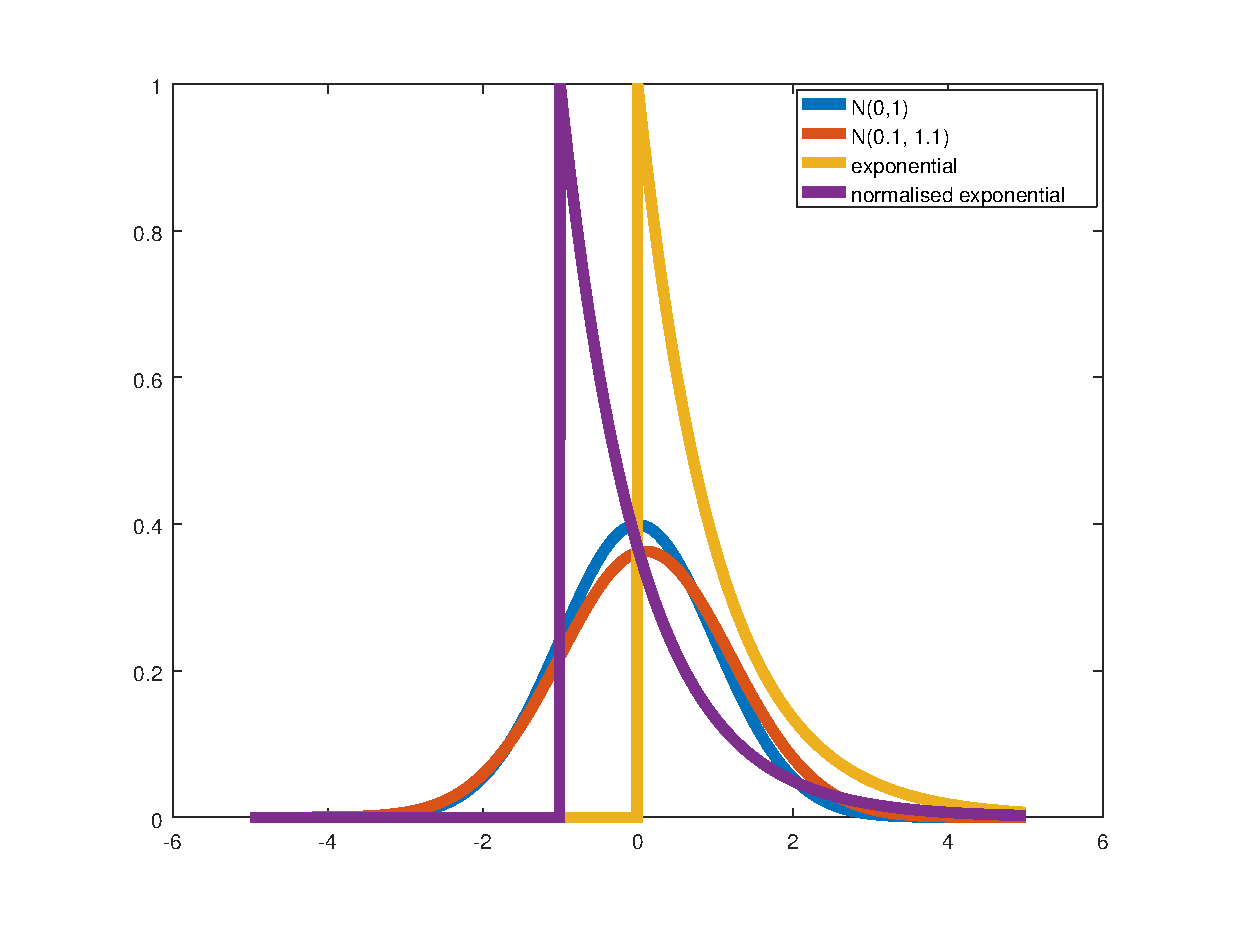
\includegraphics[width=\textwidth]{../figures/distribution_examples}
\end{frame}

\begin{frame}\frametitle{The $\chi^2$ test's performancer}
  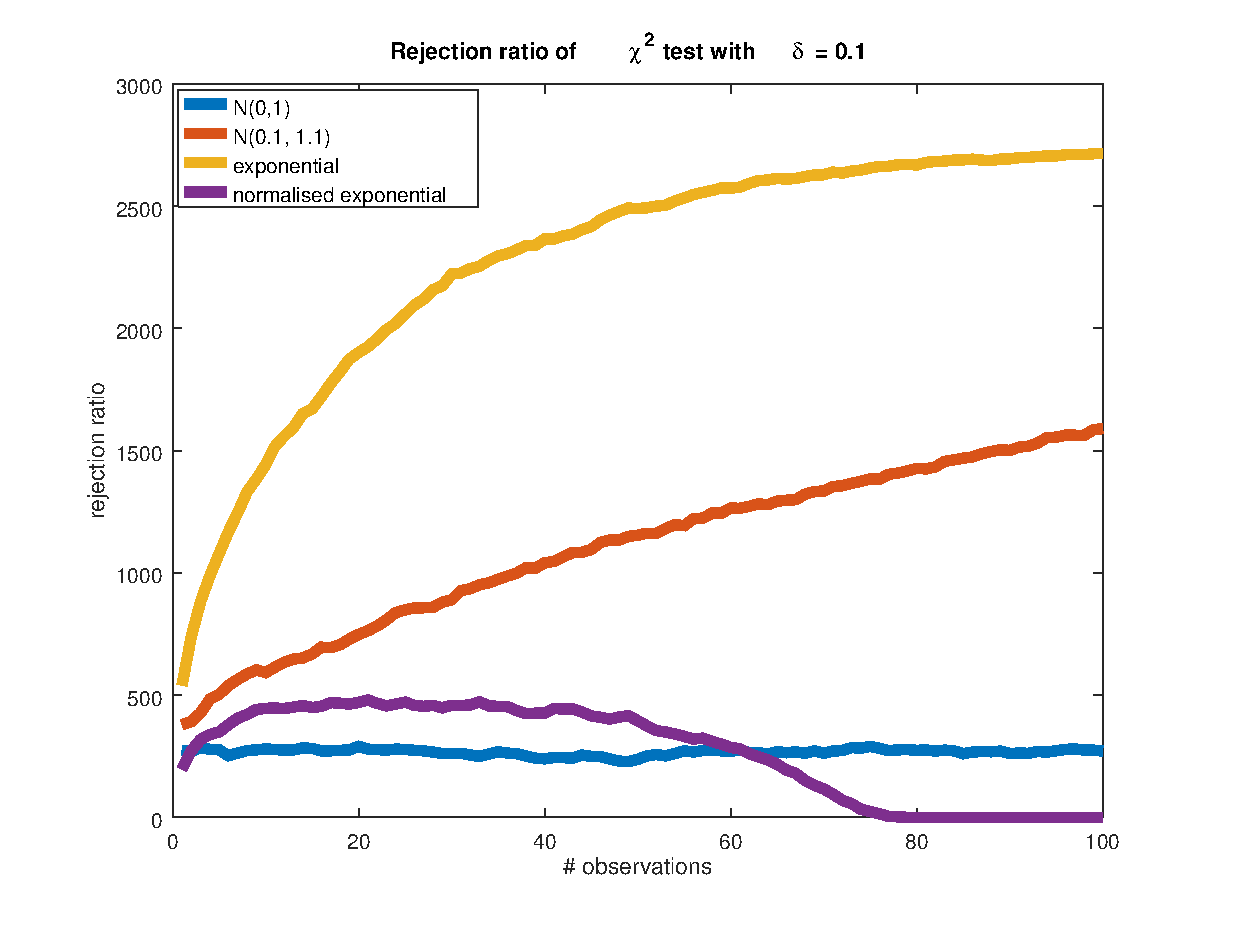
\includegraphics[width=\textwidth]{../figures/rejection_ratio}
\end{frame}





%%% Local Variables:
%%% mode: latex
%%% TeX-master: "notes"
%%% End:

